\documentclass[11pt,a4paper]{article}
\usepackage[francais]{babel}
\usepackage[utf8]{inputenc}
\usepackage[T1]{fontenc}

\usepackage{amsmath}
\usepackage{amsfonts}
\usepackage{amssymb}
\usepackage{makeidx}
\usepackage{graphicx}
\usepackage[left=1cm,right=1cm,top=1cm,bottom=2cm]{geometry}
\usepackage{tabularx}
\usepackage{epstopdf}
\usepackage{booktabs}
\usepackage{threeparttable}
\newcommand{\Angstrom}{\textup{\AA}}
\usepackage{longtable}
\usepackage{multirow}
%\usepackage[labelfont=bf]{caption}
\usepackage{multicol}
\usepackage{pbox}
%\usepackage{hyperref}
%\usepackage{cleveref}
%\usepackage[pdftex]{graphicx}
\usepackage{epstopdf}
\usepackage{float}
\usepackage{rotating}
\usepackage{array}
 
%\usepackage{lmodern}
%\usepackage{mathpazo}
%\usepackage{microtype}
%\usepackage{geometry}
\usepackage{caption}
%\usepackage{xkeyval}
%\usepackage{subfigure}
\usepackage[dvipsnames]{xcolor}
\usepackage{sectsty}
%\usepackage{selinput}
\usepackage{babel}
%\usepackage{ulem}
%\usepackage{mathtools}
\usepackage{framed}
%\graphicspath{{/Users/bertrandsiboulet/Documents/minutes/figures/}}
\DeclareGraphicsExtensions{.eps,.pdf}
 
\newcolumntype{?}{!{\vrule width 2pt}}
%\usepackage[toc,page]{appendix}
\chapterfont{\color{NavyBlue}}
%\titleformat{\chapter}[display]
%{\normalsize \huge \color{NavyBlue}}%
%{\flushright \normalsize \color{Black}}%
%{\MakeUpperCase{\chaptertitlename}\hspace{1ex}%
%{\fontfamiliy{mdugm}\fontsize{60}{60}\selectfont\thechapter}}%
%{10pt}%
%{\bfseries\huge}%
\sectionfont{\color{BrickRed}}
\subsectionfont{\color{Maroon}}
\subsubsectionfont{\color{Red}}
\paragraphfont{\color{OrangeRed}}
%\renewcommand{\familydefault}{\sfdefault}
%\usepackage{geometry}
%\usepackage{pgfplots}
\makeatletter
\renewcommand\paragraph{\@startsection{paragraph}{4}{\z@}%
{-2.5ex\@plus -1ex \@minus -.25ex}%
{1.25ex \@plus .25ex}%
{\normalfont\color{OrangeRed}\normalsize\bfseries}}
\makeatother
 
\setcounter{secnumdepth}{4}
\setcounter{tocdepth}{4}
\bibliographystyle{elsarticle-num}
 
\usepackage[automark]{scrpage2}
\setheadsepline{.4pt}
\usepackage{listings}
\makeatletter
\renewcommand\tableofcontents{%
    \@starttoc{toc}%
}
\makeatother
\renewcommand{\arraystretch}{1.2}
%commands used in my current template
\newcommand*\mycommand[1]{\texttt{\emph{#1}}}
\newcommand*{\doi}[1]{\href{http://dx.doi.org/#1}{doi: #1}}
\newcommand{\comment}[1]{\textit{\textcolor{Red}{#1}}}
\newcommand{\addref}[1]{\textit{\textcolor{Red}{Add reference!}}}
\newcommand{\sub}[1]{\textsuperscript{#1}}
 
 
\begin{document}
\begin{flushleft}
\Large \textcolor{BrickRed}{\textsc{\textbf{Travaux d'Initiative Personnelle Encadrés}}} \\
\Huge \textcolor{BrickRed}{\textsc{\textbf{Intellingence Artificielle et prévisions météorologiques }}} \\[0.5cm]
\Large \textcolor{BrickRed}{\textsc{\textbf{Concours CPGE 2021 \\[0.5 cm]}}}
\hrule \textcolor{White}{-} \\[0.1cm]
%\Large \textcolor{BrickRed}{\textsc{\textbf{Concours CPGE 2021 \\}}}
\Large \textsc{Hélène Siboulet MP} \\
\Large \textsc{Juin 2021} \\[0.5cm]
\hrule
\end{flushleft}
\section{Présentation} 
%%%%%%%%%%
La prévision consiste à prévoir, c'est-à-dire à \og voir avant\fg{}. Il s'agit donc, à partir de ce que lo'n sait à un moment donné, de savoir ce qui se passera à un moment ultérieur, avec la meilleure probabilité.En effet, à part les phénomènes déterministes, comme par exdemple le mouvement des solides à court terme, on ne peut avoir que des indications probabilistes. C'est un problème universel, qui s'applique à l'\fg{économie, la politique, la vie privée, et aussi bien sûr aux prévisions météorologiques.   \\
La prévision repose sur deux élements : des données disponibles à un moment, et des théories ou des modèles qui permettent d'utiliser ces données. \\
Les processus météorologiques sont tout à fait chaotiques. Cela signifie que des incertitudes minimes à un instant donné peuvent avoir des conséquences très fortes sur le déroulement. En fait, ces incertitudes n'empêchent pas de prévoir à court terme, par exemple pour le lendemain, mais elles rendent difficiles les prévisions au delà de deux semaines. \\
Si les processus météorologiques sont chaotiques à moyen terme, ils sont au contraire extrêmement stables dès lors que on les analyse en moyenne. Par exempler, Milankovitch a prévu que les variations de trois paramètres~-excentricité, obliquité et précession~-auraient des effets périodiques sur les glaciations. Milankovitch a fait apparaître des périodes de 20~000, 40~000 et 100~000 ans, ce qui a été confirmé expérimentalement par les mesures de $\delta O_{18}$ dans les carottes glaciaires de Vostock, en 1976. Ces résultats montrent que, en faisant des moyennes sur une centaine d'année, on a des tendances très claires d'évolution des températures, alors qu'il est difficile de prévoir la température dans deux semaines.   
 
Dans ce documents, nous allons faire un bref état de l'art des méthodes de prévision météorologiques utilisées, et proposer une méthode basée sur l'intellignce artificielle. Nous verrons que ces deux aproches sont tout à fait différentes. Nous collectons une base de données, nous élaborons une méthode avec de nombreuses variantes. Chaque variante est évaluée numériquement, c'est à dire par comparaison des prévisions avec un ensemble de données qui ont été placées en dehors des données d'entrées. 


 
\section{État de l'art}
Méthode la plus courante de prévision météo selon Jean Pailleux de Météo-France
Modélisation de l'atmosphère par :
\begin{enumerate}
\item Équation du mouvement(Newton)
\item $\frac{d\bold{V}}{dt} = \bold(g) - \frac{\bold{grad}p}{d} $
\item Équation de continuité
\item Thermodynamique
\item Équation des gaz parfaits
\item Équations de bilans de constituants: vapeur d’eau, eau liquide, ozone, etc...
\end{enumerate}

\section{Recherche de données}

Base de donnée trouvée sur  : \\
https://donneespubliques.meteofrance.fr/?fond=produit\&id\_produit=90\&id\_rubrique=32
Contient les relevés de 62 stations en France Métropolitaine et en France d’Outre mer
De 1996 à 2020  (avec certaines mesures manquantes)
Un relevé toutes les trois heures
Paramètres atmosphériques: température, humidité, direction et force du vent, pression atmosphérique, hauteur de précipitations, temps sensible, description des nuages, visibilité
Chaque fichier couvre un mois et toutes les stations

Collecte des données avec Webbot
Décompression des fichiers au format csv
Tri des données par station

\section{Analyse sur une station unique}

Extraction des données de température et d'humidité de Clermont-Ferrand au au format json
Les annees 2008, 2019 et 2020 sont retirées de la base d'entrainement et serviront de base de test\\
! donnes\_collecte/meteo\_france/analyse\_station\_unique/humidite.png\\
! donnes\_collecte/meteo\_france/analyse\_station\_unique/temperature.png\\

Comment estimer la valeur d'un ensemble de prévisions~? On calcule l'écart quadratique moyen des écarts entre nos prévisions et les températures mesurées. cela permet d'estimer la valeur des prévisions, mais à condition d'avoir une valeur de comparaison. Nous utilisons pour cette valeur les diffréences entre les quartiles 1 et 3. Calcul des Quartiles de l'humidité et de la température. En dessous du premier quartile, on trouve le quart des valeurs, et au dessus du troisièpe quartile, on trouve un quart des valeurs. 
Température : Q1 = 6.39  Q3 = 17.4  soit un intervalle de 11${}^{\circ}C$  
Humidité : 	  Q1 = 59.0  Q3 = 85.0  soit un intervalle de 26\%

* Calcul de la moyenne de la température et de l'humidité par jour et heure
Approximation de la température à un phoénomène cyclique de période un an

ecart quadratique moyen de temperature : 4.28${}^{\circ}C$
ecart quadratique moyen d'humidite : 14.8\%

* Approximation de la courbe des températures par un fonction
À priori est un phoénomène cyclique sur l'année et sur le jour
Transformée de Fourier

Hypothèse vérifiée :
Approximation par une fonction de la forme $f(t) = A cos (w1 t + \phi^1) + B cos (w2 t + \phi^2) + C$
avec $w1 = 2 \pi  et w2 = 2 \pi /365$
Et par une fonction de la forme $g(t) = A cos (w1 t + \phi^1) + B cos (w2 t + \phi^2) + C + D cos (w3 t + \phi^3)$
avec $w3 = 4 \pi$

On utilise la méthode du gradient pour trouver les coefficient :
\begin{itemize}
\item on crée une fonction écart $(u(t))$ qui calcule l'écart entre les prévisions de $u(t)$ et les valeurs de la base d'entrainement
\item on cherche à trouver le minimum de écart en fonction des paramètres donc
\item on initialise aléatoirement les paramètres
\item on dérive écart par rapport à chaque paramètre
\item on modifie chaque paramètre X en faisant X = X - dX
\item on répète les deux points précédents un grand nombre de fois
\end{itemize}


\section{Exemples Latex}
\subsection{subsection}
\subsubsection{q;,c}
%Donner un référence : \cite{Adler:1964aa}
\subsubsection{Donner des figures}
\begin{figure}
\centering
\includegraphics[width=0.48 \textwidth]{/Users/helene/Documents/TIPE/donnees_collecte/meteo_france/analyse_station_unique/temperature.png}\quad
\includegraphics[width=0.48 \textwidth]{/Users/helene/Documents/TIPE/donnees_collecte/meteo_france/analyse_station_unique/temperature.png}
\caption{\label{fig:190101Lolita} A droite : pointe AFM / surface d'eau, à gauche :  Coalescence de gouttes d'eau }
\end{figure}
%%%%%%
\begin{figure}
  \includegraphics[width=0.48 \textwidth]{/Users/helene/Documents/TIPE/TIPERedac/imagesTIPE/temperature.png}\quad
\end{figure}
\begin{figure}
  \includegraphics[width=0.48 \textwidth]{/Users/helene/Documents/TIPE/TIPERedac/imagesTIPE/temperature.png}\quad
\end{figure}
%%%%%
%%%\begin{figure}
%\centering
%\includegraphics[width=0.48 \textwidth]{/Users/siboulet/Desktop/imagesTIPE/temperature.png}\quad
%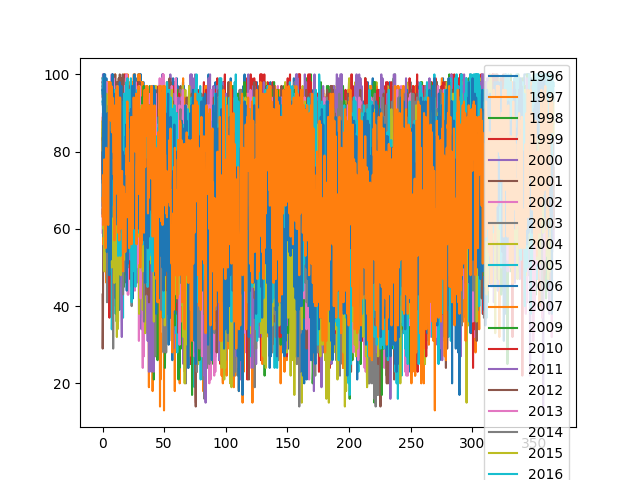
\includegraphics[width=0.48 \textwidth]{/Users/siboulet/Desktop/imagesTIPE/humidite.png}
%\caption{\label{fig:190101Lolita} A droite : pointe AFM / surface d'eau, à gauche :  Coalescence de gouttes d'eau }
%\end{figure}

\subsubsection{Citer des figures}
Je cite la figure \ref{fig:190101Lolita}
%%%%%
\subsection{Placer un tableau}
\begin{table}[ht]
\begin{tabular}{cccc}\hline
\hline
Ow& 15.99945& -0.8476&SPCE\\
Hw&  1.0079 &  0.4238&SPCE\\
Na& 22.9897 &  1.0000&\\         
Cl& 35.45   & -1.0000&\\
Os& 15.9994 & -1.000 &\\   
Ti& 47.8670 &  2.000 &\\  
\hline 
\end{tabular}                     
\caption{\label{MonTableau}, Charges for Ti02/W/Na/Cl}
\end{table}
\subsection{Citer un tableau}
Je cite mon tableau \ref{MonTableau}.


\section{Références}
%\bibliography{/Users/helene/Documents/TIPE/TIPERedac/bibH}
%\begin{enumerate}
%\item Baselov, I., Vasileva, D., 2016. Numerical modeling of drop coalescence in the presence of soluble surfactants. J. Computational and Applied Mathematics 293, 7-19.
%\item Duchemin, L., Eggers, J., Josserand, C., 2003. Inviscid coalescence of drop. J. Fluid Mech. 487, 167-178.
%\end{enumerate}

\end{document}